\documentclass[12pt,letterpaper]{article}
\usepackage[utf8]{inputenc}
\usepackage[spanish]{babel}
\usepackage{amsmath}
\usepackage{amsfonts}
\usepackage{amssymb}
\usepackage{natbib}
\usepackage{graphicx}
\usepackage{cite}
\usepackage{wrapfig}
\usepackage{afterpage}
\setcitestyle{square}
\usepackage[export]{adjustbox}
\usepackage[left=2cm,right=2cm,top=2cm,bottom=2cm]{geometry}
\usepackage{afterpage}
\usepackage{setspace}
\spanishdecimal{.}
\usepackage{hyperref}
\usepackage{float}
\usepackage{multirow} 

\author{C. Iván Pineda S.\textsuperscript{1} }
\title{Implementación de un algoritmo genético para optimizar trayectorias en un modelo del sistema solar.\\ IIMAS}
\date {\textit{\textsuperscript{1}Universidad Nacional Autónoma de México}
\\ 4 de septiembre de 2018}

\begin{document}
\maketitle

\begin{abstract}
El objetivo de este trabajo es modelar el sistema solar y su dinámica utilizando las ecuaciones de movimiento para  un sistema de $n $ cuerpos. Para darle solución a este problema de modelado se empleó un algoritmo genético con el fin de encontrar las trayectorias óptimas para el viaje desde la Tierra hasta otro cuerpo del sistema solar, la función de evaluación de dicho algoritmo recibe la velocidad inicial de la nave, un tiempo de inicio del viaje y utiliza el método de Euler para resolver las trayectorias de cada uno de los cuerpos. La evaluación es multiobjetivo y toma en cuenta la distancia más corta a la que estuvo la nave de su destino, la última distancia de la nave a su destino (en caso de que no llegase a la superficie del mismo), el tiempo que tomó realizar el viaje y el tiempo que la nave estuvo cerca del destino.
\end{abstract}


\section*{Introducción}

\subsection*{Mecánica newtoniana}

La interacción gravitatoria no relativista de dos cuerpos con masa ($m_1$ y $m_2$) se describe con la segunda ley de Newton y con la ley de gravitación universal \citep{jose2000classical}.

\begin{equation}
 m_1\dfrac{d ^2 \mathbf{(r_1 - r_2)}}{d t^2}=-G\dfrac{m_1m_2}{|\mathbf{r_{1}}-\mathbf{r_2}|^3}(\mathbf{r_{1}}-\mathbf{r_2})
\end{equation} 

Donde:
\\
\\
$G=39.4784176 \ AU^3 \ YR^{-2} \ SM^{-1}$, G es la constante de gravitación universal, AU=Unidad Astronómica, YR=Año, SM=Masas solares.
\\
\\
$\mathbf{r_n} $ es el vector de posición de cada cuerpo.
\\
\\
\\
Simplificando la ecuación (1), obtenemos una función para la aceleración (2):

\begin{equation}
 m_1\dfrac{d ^2 \mathbf{(r_1-r_2)}}{d t^2}=-G\dfrac{m_1m_2}{|\mathbf{r_{1}}-\mathbf{r_2}|^3}(\mathbf{r_{1}}-\mathbf{r_2}) \Rightarrow \dfrac{d ^2 \mathbf{(r_1-r_2)}}{d t^2}=-G\dfrac{m_2}{|\mathbf{r_{1}}-\mathbf{r_2}|^3}(\mathbf{r_{1}}-\mathbf{r_2})
\end{equation} 

La ecuación (2) determina la dinámica de un cuerpo causada por la atracción gravitacional de otro cuerpo con masa, el problema a resolver es de n cuerpos. La fuerza que siente un cuerpo en un determinado momento es la suma de las fuerzas de cada uno de los cuerpos a su alrededor exceptuándose a si mismo. Utilizando (2), esto es:

\begin{equation}
 \mathbf{a_{k}}=\sum_{i=1 , i \neq k}^{n} \dfrac{d ^2 \mathbf{(r_k-r_i)}}{d t^2}
\end{equation}

Utilizando (2) y (3) se obtiene:

\begin{equation}
  \mathbf{a_k}=\sum_{i=1 , i \neq k}^{n}[ -G\dfrac{m_i}{|\mathbf{r_{k}}-\mathbf{r_i}|^3}(\mathbf{r_{k}}-\mathbf{r_i})]=-G \sum_{i=1 , i \neq k}^{n} m_ i\dfrac{\mathbf{r_{k}}-\mathbf{r_i}}{|\mathbf{r_{k}}-\mathbf{r_i}|^3}
\end{equation}

La $k$ representa al cuerpo del cual queremos obtener la aceleración y la $i$ es cada uno de los $n$ cuerpos que influyen gravitacionalmente sobre $k$.

Utilizando el método de Euler para integrar una ecuación diferencial y así obtener la velocidad y la posición de de un cuerpo $k$ en un instante $t$, de (4) obtenemos:

\begin{equation}
 \mathbf{v_{k_{t+1}}} =  \mathbf{v_{k_t}} + \mathbf{a_k} dt = \mathbf{v_{k_t}} - G \sum_{i=1 , i \neq k}^{n} m_ i\dfrac{\mathbf{r_{k}}-\mathbf{r_i}}{|\mathbf{r_{k}}-\mathbf{r_i}|^3} dt
\end{equation}

\begin{equation}
 \mathbf{r_{k_{t+1}}} =  \mathbf{r_{k_t}} +  \mathbf{v_{k_{t+1}}} dt = \mathbf{r_{k_t}} + [\mathbf{v_{k_t}} + \mathbf{a_k} dt] dt = \mathbf{r_{k_t}} + \mathbf{v_{k_t}} dt - G \sum_{i=1 , i \neq k}^{n} m_ i\dfrac{\mathbf{r_{k}}-\mathbf{r_i}}{|\mathbf{r_{k}}-\mathbf{r_i}|^3} dt ^ 2
\end{equation}

Que son funciones para la velocidad y la aceleración de un cuerpo $k$.

\subsubsection*{Implementación en pseudocódigo}
//Una implementación para un módelo del sistemas solar basado en el método de Euler. \\
\hspace*{0.65cm}n = [Sol, Mercurio, Venus, Tierra, ..., nave] \\
\hspace*{0.5cm} for k in n: \\
\hspace*{1cm} $\mathbf{a_k} = vector(0,0,0)$ \\
\hspace*{1cm} for i in n: \\
\hspace*{1.5cm} if k!=i: \\
\hspace*{2cm} $\mathbf{a_{k}} +=  - G * m_i * \dfrac{\mathbf{r_{k}}-\mathbf{r_i}}{|\mathbf{r_{k}}-\mathbf{r_i}|^3} * dt$ \\ 
\hspace*{1.65cm}end if \\
\hspace*{1cm} end for\\
\hspace*{1.1cm}$ \mathbf{r_{k}} +=  \mathbf{v_{k}} * dt + \mathbf{a_{k}} *  dt ^2 $ \\
\hspace*{1.1cm}$ \mathbf{v_{k}} +=   \mathbf{a_{k}} * dt  $ \\
\hspace*{0.6cm} end for 

\subsection*{Algoritmos genéticos}

Los algoritmos genéticos forman parte de los métodos heurísticos de optimización y se utilizan para encontrar los máximos y/o mínimos de una función evitando las derivadas y cálculo de  gradientes, se basan en la selección natural \citep{gestal2010introduccion}.

\subsubsection*{Codificación binaria}

En la naturaleza la información necesaria para codificar las proteínas que constituyen a los seres vivos está almacenada en una cadena de ADN, dicha cadena se compone de solo 4 bases; adenina, guanina, citosina y timina. Posteriormente se realiza una transcripción a ARN que se compone de las mismas bases, solo se cambia timina por uracilo y finalmente se realiza la traducción a proteínas. 

Para este algoritmo se utilizó una codificación en números binarios, es decir, una cadena de solo 0 y 1 que posteriormente fue traducida a un número decimal que se encuentra dentro de un intervalo dado.

Se creó un número determinado de cadenas de binarios que fue nuestra población, cada una de estas cadenas tiene un número determinado de bits al que llamamos $n$ y la distribución de ceros y unos es aleatoria.

Para convertir la cadena binaria a decimal se realizó un procedimiento idéntico al del siguiente ejemplo:

\[
dec=101011_2=1*2^5+0*2^4+1*2^3+0*2^2+1*2^1+1*2^0=32+0+8+0+2+1=43
\]

Para que dicho número esté en el intervalo en el que vamos a evaluar a nuestra función utilizamos:

\begin{equation}
decInt=a+\dfrac{dec}{2^n-1}(b-a)
\end{equation}

Donde $a$ y $b$ son los límites mínimo y máximo respectivamente, $n$ es el número de bits de nuestra cadena y $dec$ es nuestra primer conversión de binario a decimal, $decInt$ es el decimal que recibe la función de evaluación.

\subsubsection*{Selección}

El objetivo es encontrar los mínimos. Por lo tanto, seleccionamos aquellas cadenas que al ser convertidas a decimal y al evaluarlas en la función $f(v_{x_0},v_{y_0},inicio)$ den los resultados más pequeños, es decir, las cadenas que produzcan las trayectorias con mejor $fitness$. La función evidentemente tiene un gran número de mínimos, obtenerlos con métodos numéricos o analíticos convencionales no es lo más efectivo.

El punto $P$ es un mínimo local de $f$ si existe un entorno reducido de centro $x_0$, que cumpla que $f(x)\geq f(x_0) \ \forall x \in E'(x_0)$. $P(x_0,f(x_0))$ es un mínimo absoluto de $ f \Longleftrightarrow \forall x \neq x_0, A, f(x_0)\leqslant f(x)$, donde $A$ es un subconjunto del dominio de $f$.

La cantidad de cadenas a seleccionar puede variar. Para este trabajo se utilizó la mitad de la población, es decir solo el 50\% más adaptado puede dejar descendencia.

\subsubsection*{Reproducción}

Una vez que se seleccionan los individuos más aptos, es necesario que dejen descendencia. Se seleccionan dos cadenas al azar, a partir de las cuales se crea una cadena hija. Para este algoritmo se genera una cantidad de cadenas hijas igual a la cantidad de cadenas padres, es decir, la mitad de la población inicial, así padres e hijos sumaran la misma cantidad de cadenas que al inicio.

Hay varias formas de combinar los genes (unidades de información, en este caso bits), aquí se utilizó el cruce uniforme que consiste en formar una cadena hija a partir de dos padres, donde cada bit de las cadenas padres tiene un 50 \% de probabilidad de pasar al hijo. Esto se logra seleccionando aleatoriamiente un bit en una posición específica de las cadenas padres (lo más fácil es empezar en la posición 0 y terminar en el último carácter de la cadena). Dicho bit se asigna en la misma posición para el hijo y se descarta esa posición.

\subsubsection*{Mutación}

Las mutaciones son esenciales para mantener la variabilidad en nuestra población, sin estas, nuestros individuos tendrán el mismo valor en un menor número de generaciones, esto es ideal sí ese valor corresponde a un mínimo, pero casi nunca es así.

Para mutar a un individuo es necesario cambiar aleatoriamente el valor de algunos de sus genes o bits, para esto se genera un número aleatorio en un intervalo que va desde el 0 hasta la longitud de la cadena menos 1, se escoge la posición en la cadena correspondiente a ese número y se intercambia su valor por 0 si era 1 y viceversa, se realiza lo mismo el número de veces que se quiera mutar al individuo y esto se repite para una cantidad aleatoria de individuos.

\subsubsection*{Algoritmo principal}

Los pasos que se llevan a cabo son los siguientes:

\ \ \ \ \ 1. Generación de una población inicial de cadenas.

\ \ \ \ \ 2. Evaluación.

\ \ \ \ \ 3. Selección de las más aptas.

\ \ \ \ \ 4. Reproducción.

\ \ \ \ \ 5. Mutación solo en los hijos.

\ \ \ \ \ 6. Generación de una nueva población que es la suma de los padres y los hijos.

\ \ \ \ \ 7. Se regresa al paso 2 con la generación obtenida en el paso 6 hasta una condición de paro 

\ \ \ \ \ \ \ \ o cuando se alcance el número específico de iteraciones.

\ \ \ \ \ 8. Se imprimen o guardan los valores de todas las generaciones.

\section*{Métodos}

Este trabajo está basado en un artículo sobre el Diseño de un programa en python para la enseñanza de la transferencia de órbita de Hohmann \citep{mendez2016diseno}.

Se utilizó python para la elaboración de los algoritmos, la librería de math y numpy para el desarrollo matemático, cython y multiprocessing para optimizar el tiempo de ejecución, random para generar números aleatorios y Visual Python para el modelo visual, el código se puede revisar en \url{https://github.com/Ivan252512/AGSistemaSolar.git}. Visual python es la única biblioteca que no se instala con Anaconda, para hacerlo es necesario ejecutar desde la terminal de Linux \textbf{pip install vpython}, para más información visitar el sitio \url{http://vpython.org} y \url{https://www.anaconda.com/}.

La velocidad del cohete varía entre 40320 km/hr (velocidad de escape para la Tierra) y 60000 km/hr. Para la simulación se agregaron 15 cuerpos, entre estos están todos los planetas del sistema solar, el Sol, 4 satélites de Júpiter, la Luna, un satélite de Saturno y la nave. Para resolver las trayectorias se utilizaron las ecuaciones (5) y (6).


\section*{Resultados}
\subsection*{Luna}


\begin{tabular}{l}
Tabla 1. Valores para la Luna \\
	\begin{tabular}{|l|l|l|l|l|l|}
	\hline
	Variable & Población & Generaciones & Tiempo total & Tiempo de inicio & dt \\	\hline 
	Valor & 40  & 70 & 30.4 días & 0-15.2 días & 1 min  \\ \hline
	\end{tabular}
\end{tabular}

\begin{figure}[H]
\centering
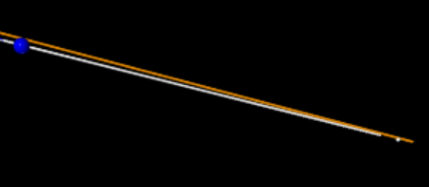
\includegraphics[width=0.8\textwidth]{luna}
\caption{Trayectoria óptima de la nave (naranja) desde la Tierra (azul) a la Luna (blanco), se encontró una ruta que llega directo a la Luna.}
\end{figure}

\begin{figure}[H]
\centering
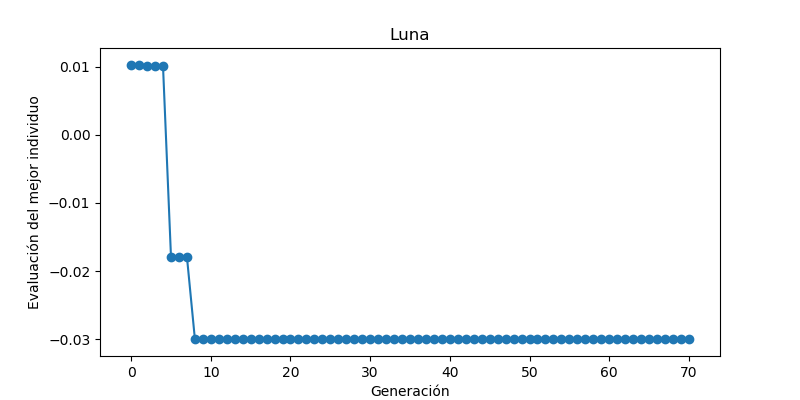
\includegraphics[width=0.8\textwidth]{Lunaind}
\caption{Gráfica que compara el resultado de la evaluación para el mejor individuo por generación contra su generación, desde la novena generación los resultados comienzan a ser constantes. }
\end{figure}

\begin{figure}[H]
\centering
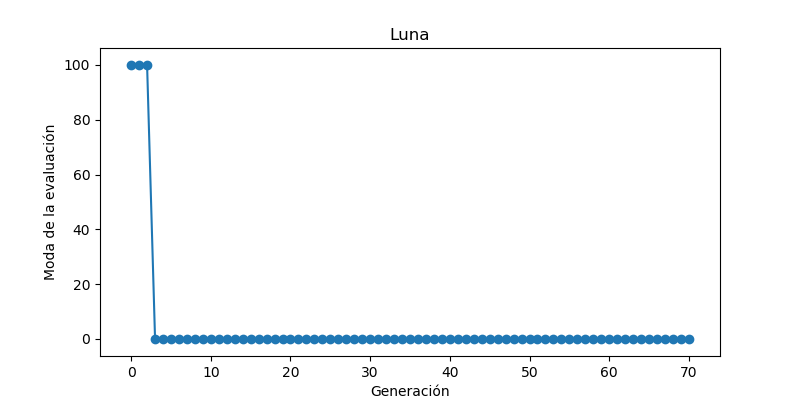
\includegraphics[width=0.8\textwidth]{Lunamoda}
\caption{Gráfica que compara el resultado de la evaluación para la moda de cada generación, los resultados son similares a los de la gráfica del mejor individuo, esto indica que se cumple que los mejores individuos son los que dejan mayor descendencia, exceptuando las primeras generaciones.}
\end{figure}

\begin{figure}[H]
\centering
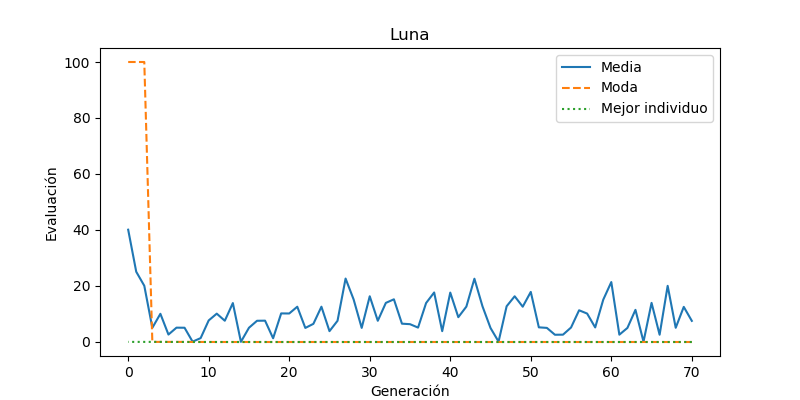
\includegraphics[width=0.8\textwidth]{Luna}
\caption{Comparación del mejor individuo, la moda y la media de cada generación.}
\end{figure}





\subsection*{Tierra}

El objetivo era lograr que la nave orbitara a la Tierra, no se logró, pero la trayectoria sí es cercana a dicho planeta. 

\begin{figure}[H]
\centering
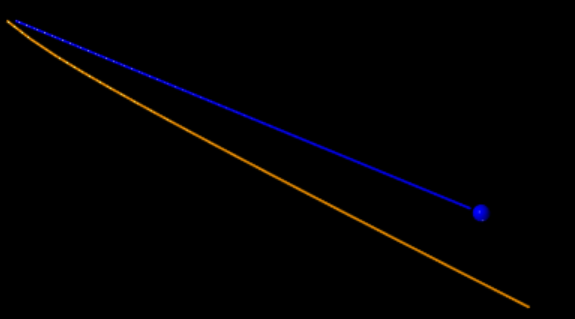
\includegraphics[width=0.8\textwidth]{tierra}
\caption{Trayectoria óptima de la nave (naranja) desde la Tierra (azul).}
\end{figure}


\begin{tabular}{l}
Tabla 1. Valores para la Tierra \\
	\begin{tabular}{|l|l|l|l|l|l|}
	\hline
	Variable & Población & Generaciones & Tiempo total & Tiempo de inicio & dt \\	\hline 
	Valor & 40  & 70 & 15.2 días & 0-7.1 días & 1 min  \\ \hline
	\end{tabular}
\end{tabular}


\begin{figure}[H]
\centering
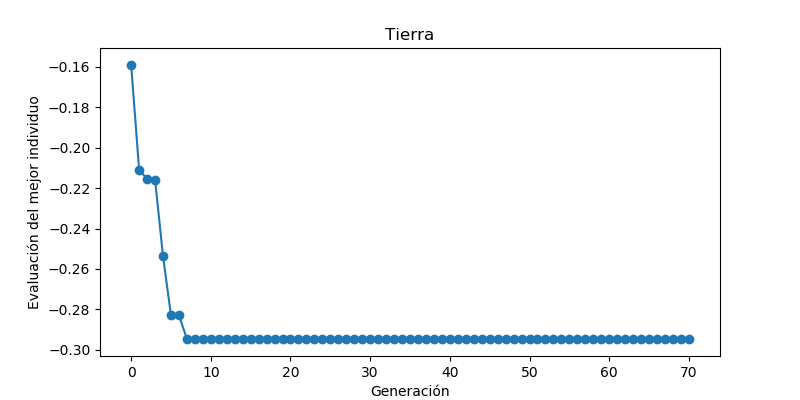
\includegraphics[width=0.8\textwidth]{Tierraind}
\caption{Gráfica que compara el resultado de la evaluación para el mejor individuo por generación contra su generación, desde la octava generación los resultados comienzan a ser constantes. }
\end{figure}

\begin{figure}[H]
\centering
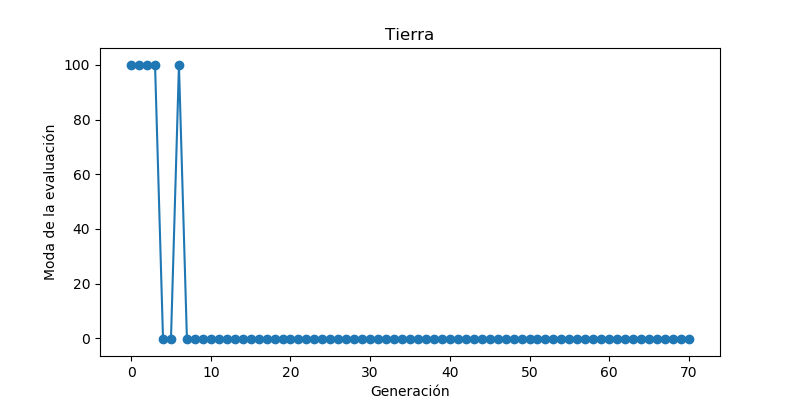
\includegraphics[width=0.8\textwidth]{Tierramoda}
\caption{Gráfica que compara el resultado de la evaluación para la moda de la generación, los resultados son similares a los de la gráfica del mejor individuo, esto indica que se cumple que los mejores individuos son los que dejan mayor descendencia, exceptuando las primeras generaciones.}
\end{figure}

\begin{figure}[H]
\centering
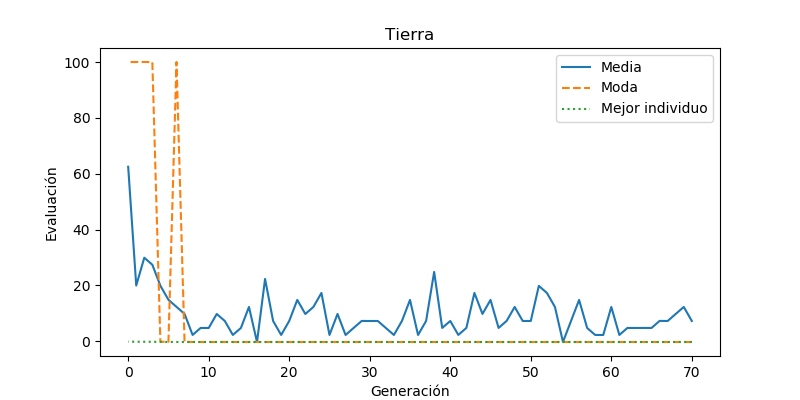
\includegraphics[width=0.8\textwidth]{Tierra}
\caption{Comparación del mejor individuo, la moda y la media de cada generación.}
\end{figure}


\subsection*{Júpiter}

Para lograr trayectorias largas en un tiempo factible es necesario usar dt grandes, por lo que la propagación de errores es también significativa.

\begin{figure}[H]
\centering
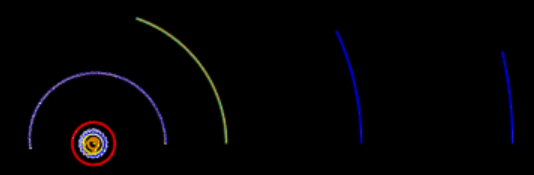
\includegraphics[width=0.8\textwidth]{jupiter}
\caption{Trayectoria óptima de la nave (naranja) desde la Tierra (azul) a Júpiter(Verde), no se acerca la nave, las órbitas en general son muy erradas por el dt.}
\end{figure}


\begin{tabular}{l}
Tabla 1. Valores para Júpiter \\
	\begin{tabular}{|l|l|l|l|l|l|}
	\hline
	Variable & Población & Generaciones & Tiempo total & Tiempo de inicio & dt \\	\hline 
	Valor & 20  & 20 & 10 años & 0-5 años & 100 min  \\ \hline
	\end{tabular}
\end{tabular}


\begin{figure}[H]
\centering
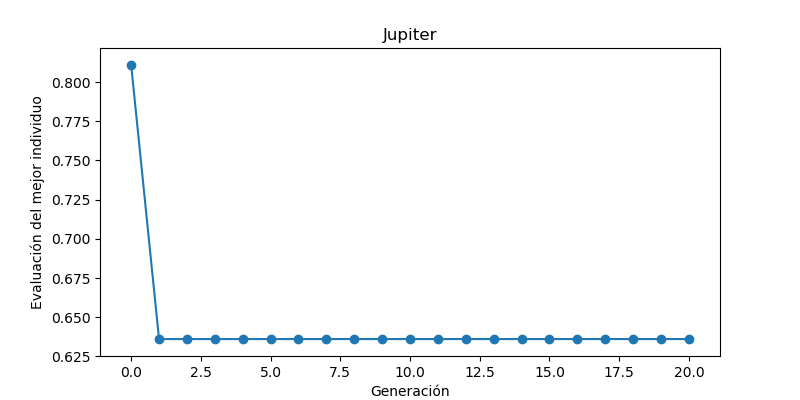
\includegraphics[width=0.8\textwidth]{Jupiterind}
\caption{Gráfica que compara el resultado de la evaluación para el mejor individuo por generación contra su generación, desde la segunda generación los resultados comienzan a ser constantes. }
\end{figure}

\begin{figure}[H]
\centering
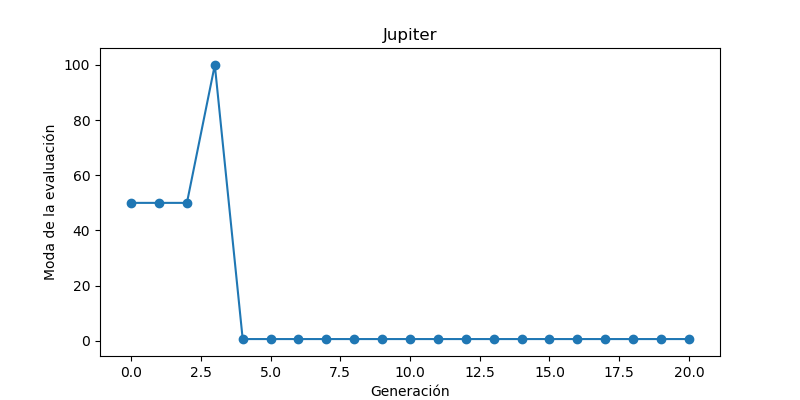
\includegraphics[width=0.8\textwidth]{Jupitermoda}
\caption{Gráfica que compara el resultado de la evaluación para la moda de la generación, los resultados son similares a los de la gráfica del mejor individuo, esto indica que se cumple que los mejores individuos son los que dejan mayor descendencia, exceptuando las primeras generaciones.}
\end{figure}

\begin{figure}[H]
\centering
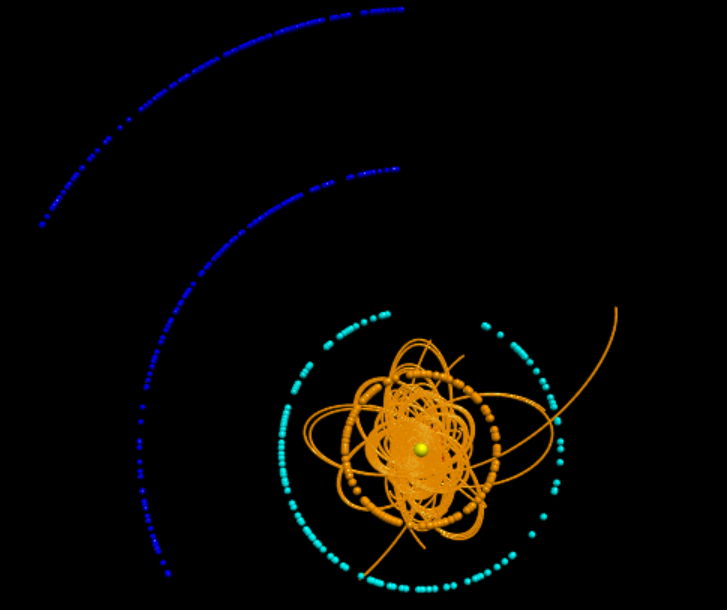
\includegraphics[width=0.8\textwidth]{Jupiter}
\caption{Comparación del mejor individuo, la moda y la media de cada generación.}
\end{figure}


\section*{Conclusiones}

Los algoritmos genéticos son una herramienta potente para problemas de optimización. Sin embargo, dado que se necesita realizar repetidamente la evaluación para cada uno de los individuos y para varias generaciones, el tiempo de computo puede llegar a ser insostenible, todo depende de la complejidad en tiempo del algoritmo y principalmente de la función de evaluación. En el caso de la implementación de este problema, se almacenaron en memoria durante el tiempo de ejecución los datos conforme se iban evaluando, para el momento en el que se tenían cerca de 2000 individuos se utilizaban cerca de 12 Gb, una buena optimización a futuro sería hacer persistentes los datos conforme va terminando cada generación, así se evitaría utilizar toda la RAM del equipo.

Es aconsejable utilizar los algoritmos genéticos cuando los métodos «precisos» no se puedan implementar correctamente , aunque los AG pueden optimizar, no siempre encuentran los mínimos o máximos absolutos, esto es algo a tomar en cuenta a la hora de solucionar un problema, hay métodos que ayudan a no estancarse en puntos críticos relativos y de ser posible deben implementarse, pero si se puede hacer un mapeo o encontrar de forma analítica dichos puntos deberían contemplarse estas opciones sobre los AG. 

\bibliography{TrabajoFinal}
\bibliographystyle{apa}

\end{document}

